\documentclass[11pt]{article}
\usepackage[a4paper, margin=2.5cm]{geometry}
\usepackage{graphicx}
\usepackage{caption}
\usepackage{amsmath} 
\usepackage{pdfcomment}
\usepackage{float}
\usepackage{tikz}
\usepackage{listings}
\usepackage{xcolor} % dla kolorowania składni
\usepackage[polish]{babel}
\usepackage[utf8]{inputenc}
\usepackage[T1]{fontenc}
\captionsetup{font=small, skip=6pt}
\usepackage{titlesec}
\usepackage{parskip}
\setlength{\parskip}{4pt}
\setlength{\textfloatsep}{10pt}
\setlength{\floatsep}{6pt}
\setlength{\intextsep}{10pt}

\lstdefinelanguage{Ccustom}{
  language=C,
  morekeywords={uint16_t, bldc_position_t, bldc_direction_t, bldc_commutation_t, inline,
  BLDC_DIRECTION_FORWARD, BLDC_DIRECTION_BACKWARD, BLDC_POSITION_0, BLDC_POSITION_60, BLDC_POSITION_120, BLDC_POSITION_180,BLDC_POSITION_240,BLDC_POSITION_300},
  sensitive=true,
}

\lstset{
  language=Ccustom,
  basicstyle=\ttfamily\small,
  keywordstyle=\color{blue}\bfseries,
  stringstyle=\color{orange},
  commentstyle=\color{gray},
  numberstyle=\tiny\color{gray},
  numbers=left,
  stepnumber=1,
  numbersep=10pt,
  backgroundcolor=\color{white},
  frame=single,
  tabsize=4,
  showspaces=false,
  showstringspaces=false,
  breaklines=true,
  breakatwhitespace=true,
  captionpos=b
}

\titlespacing*{\section}{0pt}{2ex plus .2ex minus .2ex}{1ex plus .2ex}
\titlespacing*{\subsection}{0pt}{1ex plus .1ex minus .1ex}{0.5ex plus .1ex}

\usepackage{parskip}
\setlength{\parskip}{2pt}

\title{Silnik bezszczotkowy prądu stałego (BLDC). Model i komutacja elektroniczna.}

\author{
  Paweł Michalski \\
  Mateusz Jaworski \\
  Piotr Migdałek \\
  Jakub Jaszczak \\
  Franciszek Janicki
}

\begin{document}

\maketitle

\tableofcontents
\newpage

\section{Na podstawie udostępnionych materiałów i wprowadzenia przeprowadzić analizę działania modelu silnika.}


Silnik BLDC (bezszczotkowy silnik prądu stałego) składa się ze stojana z uzwojeniami (cewkami), wirnika z magnesami trwałymi oraz opcjonalnie czujników położenia, które wspomagają sterownik w odpowiednim zasilaniu uzwojeń.

\medskip
\noindent
\textbf{Wirnik} jest połączony z wałem, do którego przymocowane są magnesy trwałe. Magnesy ustawione są naprzemiennie (bieguny N, S, N, S itd.) wokół wirnika. Liczba magnesów zależy od konstrukcji silnika i wpływa na charakterystykę pracy maszyny. 

\medskip
\noindent
\textbf{Stojan} zawiera cewki nawinięte na rdzenie z materiału ferromagnetycznego oraz cienkie blaszki. Zwiększenie liczby biegunów powoduje wzrost momentu obrotowego i jednocześnie spadek prędkości obrotowej. Dla \( n \) biegunów moment jest około \( n \) razy większy, a prędkość \( n \) razy mniejsza w porównaniu z maszyną z jednym biegunem.

Cewki, zbudowane z miedzianych drutów, są połączone w układ trójfazowy (fazy A, B, C). Końce uzwojeń stojana łączy się w gwiazdę.

\begin{figure}[H]
\centering
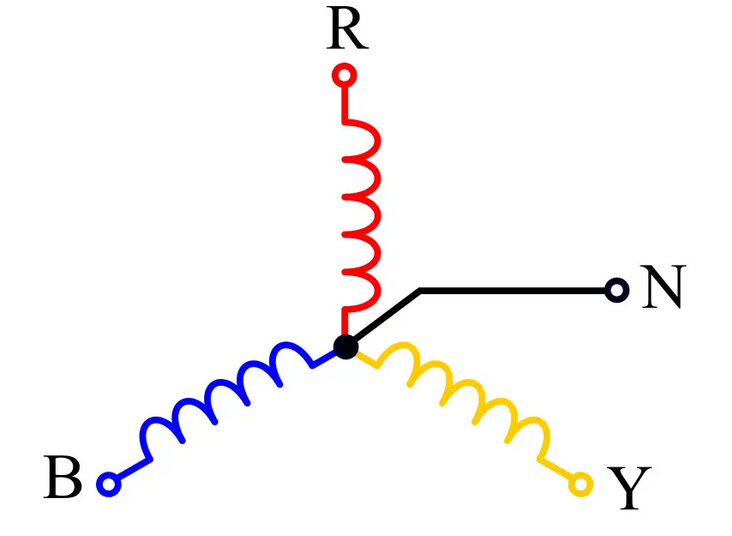
\includegraphics[width=0.8\textwidth]{aun2_star_connection.png}
\caption{Schemat polaczenia w gwiazde}
\end{figure}

\medskip
\noindent
\textbf{Zasada działania i sterowanie}

Podczas pracy silnika BLDC wykorzystywane są dwie fazy jednocześnie, przez które płynie prąd o jednakowej wartości. Silnik ten różni się od klasycznego silnika DC z komutatorem tym, że wymaga sterownika elektronicznego i nie posiada szczotek.

W uzwojeniach nieaktywnych podczas obrotu wirnika indukuje się napięcie zwrotne (napięcie wsteczne, back-EMF), które umożliwia sterownikowi ocenę prędkości kątowej i odpowiednie dopasowanie sekwencji zasilania faz. Alternatywnie można stosować czujniki Halla do detekcji położenia wirnika i synchronizacji sterowania.

Podobnie jak w silniku DC, wirujące pole magnetyczne generowane przez elektromagnesy stojana oddziałuje z polem magnesów trwałych wirnika, co powoduje jego obrót.

\begin{figure}[H]
\centering
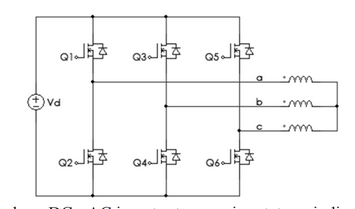
\includegraphics[width=0.8\textwidth]{aun2_3phase_bridge.png}
\caption{Schemat mostka trojfazowego do sterowania silnikiem BLDC}
\end{figure}

\medskip
\noindent
Silnik BLDC generuje trapezoidalne napięcie wsteczne (back-EMF), co ma wpływ na sposób sterowania i pomiaru.

\section*{Model silnika BLDC}

Modelowanie silnika BLDC opiera się na podobnych zasadach jak modelowanie silników prądu stałego, uwzględniając zarówno równania elektryczne, jak i mechaniczne. Różnice wynikają z konstrukcji maszyny:

\begin{itemize}
    \item Uzwojenia fazowe stojana są symetryczne i skoncentrowane, dlatego rezystancje i indukcyjności stojana są stałe i równe, a indukcyjność wzajemna każdej cewki jest pomijana.
    \item Straty histerezy i prądów wirowych są pominięte, a nasycenie magnetyczne jest zaniedbane.
    \item Nie uwzględnia się reakcji twornika.
\end{itemize}

\begin{figure}[H]
\centering
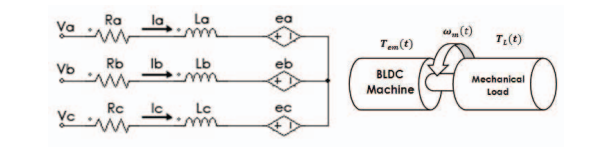
\includegraphics[width=0.8\textwidth]{aun2_bldc_schematic.png}
\caption{Schemat elektryczny silnika BLDC}
\end{figure}

Model elektryczny można rozpatrywać dla pojedynczej fazy uzwojeń stojana.

\begin{equation}
v_{k,n}(t) = R i_k(t) + L \frac{di_k}{dt}(t) + e_k(t)
\label{eq:voltage}
\end{equation}

gdzie:
\begin{itemize}
\item $v_{k,n}(t)$ - chwilowe napięcie fazy $k$
\item $i_k(t)$ - chwilowy prąd fazy $k$
\item $e_k(t)$ - chwilowe napięcie wsteczne fazy $k$
\item $R$ - rezystancja każdego uzwojenia stojana
\item $L$ - indukcyjność każdego uzwojenia stojana
\end{itemize}

Równanie ruchu mechanicznego silnika BLDC:

\begin{equation}
T_{em}(t) = J \frac{d\omega_m(t)}{dt} + B \omega_m(t) + T_L(t)
\label{eq:mechanical}
\end{equation}

gdzie:
\begin{itemize}
\item $T_{em}(t)$ - całkowity moment elektromagnetyczny [Nm]
\item $J$ - moment bezwładności [kg$\cdot$m$^2$]
\item $\omega_m(t)$ - mechaniczna prędkość kątowa wirnika [rad/s]
\item $B$ - współczynnik tarcia lepkiego [N$\cdot$m$\cdot$s/rad]
\item $T_L(t)$ - moment obciążenia [Nm]
\end{itemize}

Moment i napięcie wsteczne dla każdej fazy:

\begin{align}
T_{em,k} &= i_k(t) \cdot k_{T,k}(\theta_e) \label{eq:phase_torque} \\
e_k(t) &= k_{e,k}(\theta_e) \cdot \omega_m(t) \label{eq:back_emf}
\end{align}

gdzie:
\begin{itemize}
\item $k_{T,k}(\theta)$ - współczynnik momentu
\item $k_{e,k}(\theta)$ - współczynnik napięcia wstecznego
\item $\omega_m(t)$ - prędkość kątowa wirnika
\end{itemize}

Współczynnik momentu $k_{T,k}(\theta)$ można przyjąć jako równoważny współczynnikowi napięcia wstecznego $k_{e,k}(\theta)$.

\begin{figure}[H]
\centering
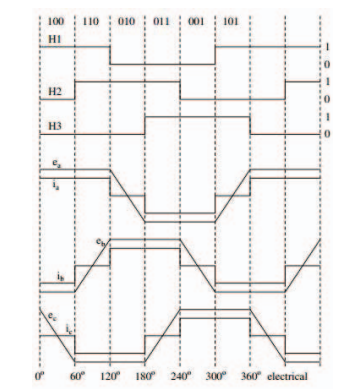
\includegraphics[width=0.8\textwidth]{aun2_trapezoid_chart.png}
\caption{Przebiegi sygnalow z czujnikow HALLa rozmieszczonych co 120 stopni i odpowiadajace im przebiegi pradu oraz napiecia faz}
\end{figure}

\medskip
\noindent
Moc silnika można opisać wzorem:
\[
P = R i^2 + \varepsilon i,
\]
gdzie \( R \) to rezystancja, \( i \) prąd, a \( \varepsilon \) jest napięciem wstecznym (back-EMF).

\medskip
\noindent
Zmianę prędkości obrotowej realizuje się przez zmianę prądu, a więc odpowiednio zmieniając napięcie zasilające.

Silnik BLDC porusza się w jednym kierunku, niezależnie od kierunku prądu, ponieważ ujemny prąd jest powiązany z ujemnym napięciem wstecznym \(\varepsilon\).


\section{Porównać przebiegi: prądu oraz generowanego momentu elektromagnetycznego dla dwóch rozkładów indukowanej SEM (badania w otwartym torze sterowania napięciem).}

\section{Wykreślić charakterystykę mechaniczną i sterowania silnika BLDC w układzie z przekształtnikiem oraz komutacją elektroniczną}

\section{Na bazie pliku źródłowego programu języka C oraz zamieszczonych oscylogramów napisać kod odpowiadający procesowi komutacji elektronicznej.}

Przeanalizowano pozycje poszczegolnych czujnikow Halla na podstawie oscylogramow i stwierdzono, ze czujnik H1 odpowiada fazie V, czujnik H2 odpowiada fazie W, natomiast czujnik H3 odpowiada fazie U\\

\begin{table}[H]
\centering
\begin{tabular}{|c|c|c|c|c|c|}
\hline
Pozycja [°] & Hall & Faza U & Faza V & Faza W \\
\hline
0 & 101 & 0 & + & - \\
\hline
60 & 100 & - & + & 0 \\
\hline
120 & 110 & - & 0 & + \\
\hline
180 & 010 & 0 & - & + \\
\hline
240 & 011 & + & - & 0 \\
\hline
300 & 001 & + & 0  & - \\
\hline
\end{tabular}
\caption{Komutacja BLDC do przodu}
\end{table}

\begin{table}[H]
\centering
\begin{tabular}{|c|c|c|c|c|}
\hline
Pozycja [°] & Hall & Faza U & Faza V & Faza W \\
\hline
0  & 101 & 0 & - & + \\
\hline
60 & 100 & + & - & 0 \\
\hline
120 & 110 & + & 0 & - \\
\hline
180 & 010 & 0 & + & - \\
\hline
240 & 011 & - & + & 0 \\
\hline
300 & 001 & - & 0 & + \\
\hline
\end{tabular}
\caption{Komutacja BLDC do tyłu}
\end{table}

\textbf{Tryb bipolarny:}
\begin{itemize}
\item Znak \texttt{+} oznacza sygnał PWM podawany na górny tranzystor.
\item Znak \texttt{-} oznacza sygnał PWM podawany na dolny tranzystor.
\item Znak \texttt{0} oznacza, że faza jest wyłączona (oba tranzystory nieprzewodzące).
\end{itemize}

textbf{Tryb unipolarny:}
\begin{itemize}
\item Znak \texttt{+} oznacza sygnał PWM podawany na górny tranzystor.
\item Znak \texttt{-} oznacza wysoki stan logiczny podawany na dolny tranzystor.
\item Znak \texttt{0} oznacza, że faza jest wyłączona (oba tranzystory nieprzewodzące).
\end{itemize}

\begin{table}[H]
\centering
\begin{tabular}{|c|c|c|c|c|c|c|c|c|}
\hline
Pozycja [°] & Hall & Ugórny & Udolny & Vgórny & Vdolny & Wgórny & Wdolny \\
\hline
0   & 101 & 0 & 0 & 1 & 0 & 0 & 1 \\
\hline
60  & 100 & 0 & 1 & 1 & 0 & 0 & 0 \\
\hline
120 & 110 & 0 & 1 & 0 & 0 & 1 & 0 \\
\hline
180 & 010 & 0 & 0 & 0 & 1 & 1 & 0 \\
\hline
240 & 011 & 1 & 0 & 0 & 1 & 0 & 0 \\
\hline
300 & 001 & 1 & 0 & 0 & 0 & 0 & 1 \\
\hline
\end{tabular}
\caption{Stany tranzystorow przy komutacji BLDC do przodu}
\end{table}

\begin{table}[H]
\centering
\begin{tabular}{|c|c|c|c|c|c|c|c|c|}
\hline
Pozycja [°] & Hall & Ugórny & Udolny & Vgórny & Vdolny & Wgórny & Wdolny \\
\hline
0   & 101 & 0 & 0 & 0 & 1 & 1 & 0 \\
\hline
60  & 100 & 1 & 0 & 0 & 1 & 0 & 0 \\
\hline
120 & 110 & 1 & 0 & 0 & 0 & 0 & 1 \\
\hline
180 & 010 & 0 & 0 & 1 & 0 & 0 & 1 \\
\hline
240 & 011 & 0 & 1 & 1 & 0 & 0 & 0 \\
\hline
300 & 001 & 0 & 1 & 0 & 0 & 1 & 0 \\
\hline
\end{tabular}
\caption{Stany tranzystorow przy komutacji BLDC do tyłu}
\end{table}

Dla sterowania bipolarnego sygnał PWM podajemy zarówno na górny, jak i dolny tranzystor oznaczony „1”.

W trybie unipolarnym dla górnego tranzystora oznaczonego „1” podajemy sygnał PWM, natomiast dolny tranzystor w tym samym czasie otrzymuje stan logiczny „1”.\\

\section*{Sterowanie przy użyciu kanałów komplementarnych PWM}

Aby ograniczyć liczbę używanych kanałów PWM do trzech (po jednym na każdą fazę), zastosowano tryb komplementarny PWM. W tym trybie każda faza jest sterowana jednym kanałem PWM z wyjściem głównym i komplementarnym. Kanał główny steruje górnym tranzystorem, natomiast kanał komplementarny dolnym.

Ponieważ zarówno kanał główny, jak i komplementarny korzystają z tego samego rejestru CCR (Capture/Compare), nie ma możliwości niezależnego sterowania stanem obu tranzystorów w danej fazie. 

Z tego powodu, aby wymusić wyłączenie jednego z tranzystorów (np. dolnego, gdy górny przewodzi), stosuje się dynamiczną rekonfigurację pinu GPIO z trybu \texttt{AF} (Alternate Function - wykorzystywanego przez sygnał PWM) na \texttt{Output}, i odwrotnie. W innym wypadku nastapiłoby zwarcie.

Dzięki temu można niezależnie kontrolować stan tranzystorów pomimo wspólnego rejestru CCR.\\

Dla oszczędności miejsca w raporcie zamieszczono tylko fragment kodu źródłowego, który został uzupełniony. Funkcja sterująca silnikiem BLDC została zmodyfikowana poprzez zastąpienie instrukcji \texttt{switch} mapowaniem 3-bitowej wartości z czujników Halla na wskaźnik do odpowiedniej funkcji komutacji. Funkcjonalność programu pozostała bez zmian, natomiast rozwiązanie to pozwala na redukcję ilości kodu.\\

\begin{lstlisting}[language=Ccustom, caption=Fragment programu w C99 realizujacy sterowanie silnikiem BLDC]
typedef enum {
    BLDC_DIRECTION_FORWARD,
    BLDC_DIRECTION_BACKWARD,
} bldc_direction_t;

typedef enum {
    BLDC_POSITION_0 = 0b101,
    BLDC_POSITION_60 = 0b100,
    BLDC_POSITION_120 = 0b110,
    BLDC_POSITION_180 = 0b010,
    BLDC_POSITION_240 = 0b011,
    BLDC_POSITION_300 = 0b001,
} bldc_position_t;

#ifdef BLDC_BIPOLAR_CONTROL
// TUTAJ BIPOLARNE

static inline void bldc_commutation_forward_0(uint16_t compare)
{
    pwm_confVH(compare);
    pwm_confWL(compare);
}

static inline void bldc_commutation_forward_60(uint16_t compare)
{
    pwm_confVH(compare);
    pwm_confUL(compare);
}

static inline void bldc_commutation_forward_120(uint16_t compare)
{
    pwm_confWH(compare);
    pwm_confUL(compare);
}

static inline void bldc_commutation_forward_180(uint16_t compare)
{
    pwm_confWH(compare);
    pwm_confVL(compare);
}

static inline void bldc_commutation_forward_240(uint16_t compare)
{
    pwm_confUH(compare);
    pwm_confVL(compare);
}

static inline void bldc_commutation_forward_300(uint16_t compare)
{
    pwm_confUH(compare);
    pwm_confWL(compare);
}

static inline void bldc_commutation_backward_0(uint16_t compare)
{
    pwm_confWH(compare);
    pwm_confVL(compare);
}

static inline void bldc_commutation_backward_60(uint16_t compare)
{
    pwm_confUH(compare);
    pwm_confVL(compare);
}

static inline void bldc_commutation_backward_120(uint16_t compare)
{
    pwm_confWH(compare);
    pwm_confUL(compare);
}

static inline void bldc_commutation_backward_180(uint16_t compare)
{
    pwm_confVH(compare);
    pwm_confWL(compare);
}

static inline void bldc_commutation_backward_240(uint16_t compare)
{
    pwm_confUH(compare);
    pwm_confVL(compare);
}

static inline void bldc_commutation_backward_300(uint16_t compare)
{
    pwm_confWH(compare);
    pwm_confUL(compare);
}

#else 
// TUTAJ UNIPOLARNE

static inline void bldc_commutation_forward_0(uint16_t compare)
{
    pwm_confVH(compare);
    pwm_set_H_WL();
}

static inline void bldc_commutation_forward_60(uint16_t compare)
{
    pwm_confVH(compare);
    pwm_set_H_UL();
}

static inline void bldc_commutation_forward_120(uint16_t compare)
{
    pwm_confWH(compare);
    pwm_set_H_UL();
}

static inline void bldc_commutation_forward_180(uint16_t compare)
{
    pwm_confWH(compare);
    pwm_set_H_VL();
}

static inline void bldc_commutation_forward_240(uint16_t compare)
{
    pwm_confUH(compare);
    pwm_set_H_VL();
}

static inline void bldc_commutation_forward_300(uint16_t compare)
{
    pwm_confUH(compare);
    pwm_set_H_WL();
}

static inline void bldc_commutation_backward_0(uint16_t compare)
{
    pwm_confWH(compare);
    pwm_set_H_VL();
}

static inline void bldc_commutation_backward_60(uint16_t compare)
{
    pwm_confUH(compare);
    pwm_set_H_VL();
}

static inline void bldc_commutation_backward_120(uint16_t compare)
{
    pwm_confWH(compare);
    pwm_set_H_UL();
}

static inline void bldc_commutation_backward_180(uint16_t compare)
{
    pwm_confVH(compare);
    pwm_set_H_WL();
}

static inline void bldc_commutation_backward_240(uint16_t compare)
{
    pwm_confUH(compare);
    pwm_set_H_VL();
}

static inline void bldc_commutation_backward_300(uint16_t compare)
{
    pwm_confWH(compare);
    pwm_set_H_UL();
}

#endif

typedef void (*bldc_commutation_t)(uint16_t);

static void bldc_commutation_forward(bldc_position_t position, uint16_t compare)
{
    static bldc_commutation_t forward_commutations[] = {
        [BLDC_POSITION_0] = &bldc_commutation_forward_0,
        [BLDC_POSITION_60] = &bldc_commutation_forward_60,
        [BLDC_POSITION_120] = &bldc_commutation_forward_120,
        [BLDC_POSITION_180] = &bldc_commutation_forward_180,
        [BLDC_POSITION_240] = &bldc_commutation_forward_240,
        [BLDC_POSITION_300] = &bldc_commutation_forward_300,
    };

    if (position > 0b000 && position < 0b111) {
        forward_commutations[position](compare);
    }
}

static void bldc_commutation_backward(bldc_position_t position, uint16_t compare)
{
    static bldc_commutation_t backward_commutations[] = {
        [BLDC_POSITION_0] = &bldc_commutation_backward_0,
        [BLDC_POSITION_60] = &bldc_commutation_backward_60,
        [BLDC_POSITION_120] = &bldc_commutation_backward_120,
        [BLDC_POSITION_180] = &bldc_commutation_backward_180,
        [BLDC_POSITION_240] = &bldc_commutation_backward_240,
        [BLDC_POSITION_300] = &bldc_commutation_backward_300,
    };

    if (position > 0b000 && position < 0b111) {
        backward_commutations[position](compare);
    }
}

static void bldc_commutation(bldc_direction_t direction, uint16_t compare)
{
    static uint8_t prev_position = 0xFFU;

    uint8_t hall_1 = hall_read_H1() & 0x01U;
    uint8_t hall_2 = hall_read_H2() & 0x01U;
    uint8_t hall_3 = hall_read_H3() & 0x01U;
    uint8_t position = (hall_3 << 2U) | (hall_2 << 1U) | hall_1;

    if (position != prev_position) {
        pwm_set_L_all();

        switch (direction) {
            case BLDC_DIRECTION_FORWARD:
                bldc_commutation_forward(position, compare);
                break;
            case BLDC_DIRECTION_BACKWARD:
                bldc_commutation_backward(position, compare);
                break;
            default:
                break;
        }
    }

    prev_position = position;
}
\end{lstlisting}


\end{document}
